\chapter{Methodology}

\section{Image Alignment}

Due to various factors, recording a video with a portable handheld device can be challenging. One of the most significant difficulties is keeping the device stable while recording. The device's handheld nature makes it susceptible to movement and shakiness, which can cause a non-static video that significantly affects the accuracy of the calculated results. This section will discuss overcoming this problem by utilizing a feature detection algorithm.


\subsection{Scale Invariant Feature Transform (SIFT)}
\label{sec:sift}

Many image processing and computer vision algorithms require feature detection in input data, such as object tracking and recognition. Researchers have proposed several algorithms for feature detection, including the Harris corner detector \cite{harris1988}, the SIFT algorithm \cite{lowe2004}, and the SURF algorithm \cite{bay2006}. One significant advantage of Lowe's approach is its ability to detect and describe local features in images insensitive to scale, rotation, and illumination changes. \cite{lowe2004}.

\begin{figure}[t]
	\centering
		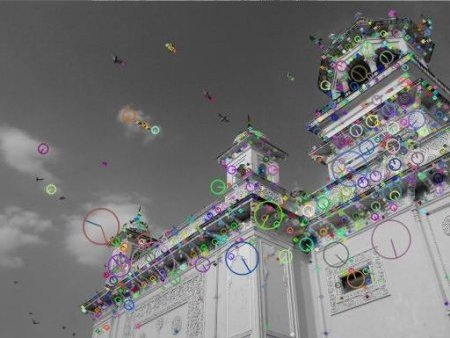
\includegraphics[scale=0.75]{texs/chapter2/image/sift1.png}
		\caption{Example of SIFT algorithm result \cite{cvSift}}
		\label{siftexample}
\end{figure}

